%%
%% プリアンブル
%%==============================================================================================================================%%
\RequirePackage{fix-cm}
%%
%% ドキュメントクラスとオプションの指定
%%--------------------------------------------------------------------------------------------------------------------%%
\documentclass[10pt,a4paper,disablejfam,dvipdfmx,fleqn,onecolumn,oneside,openany,report]{jsbook}
%%
%% パッケージの読み込み
%%--------------------------------------------------------------------------------------------------------------------%%
\input{/usr/local/etc/Package}
%%
%% コマンドと環境の定義
%%--------------------------------------------------------------------------------------------------------------------%%
\input{/usr/local/etc/Defines}
%%
%% ページレイアウト設定(A4横組用レイアウト for jsreport)
%%--------------------------------------------------------------------------------------------------------------------%%
\input{/usr/local/etc/Layouts}
%%
%% タイトル・著者名・作成日の設定
%%--------------------------------------------------------------------------------------------------------------------%%
\title{HTML5/CSS3モダンコーディング\\\small{フロントエンドエンジニアが教える3つの本格レイアウト\\\small{(写経版)}}}
\author{姫 伯邑考} \date{2020年09月01日}
%%
%% 本文
%%==============================================================================================================================%%
\begin{document}
\maketitle
%% %%
%% 部:イントロダクション
%%------------------------------------------------------------------------------------------------------------------------------%%
\part{イントロダクション}
%%
%% 章:本稿で作成するサイト
%%------------------------------------------------------------------------------------------------------------------------------%%
\chapter{本稿で作成するサイト}
%%
%% 節:Part1:スタンダードレイアウト
%%--------------------------------------------------------------------------------------------------------------------%%
\section{Part1:スタンダードレイアウト}
Web サイトに一番多く見られるベーシックなレイアウトのサイトを作成する。
\vspc{-5.00pt}\begin{figure}[H]\centering\scalebox{0.48}{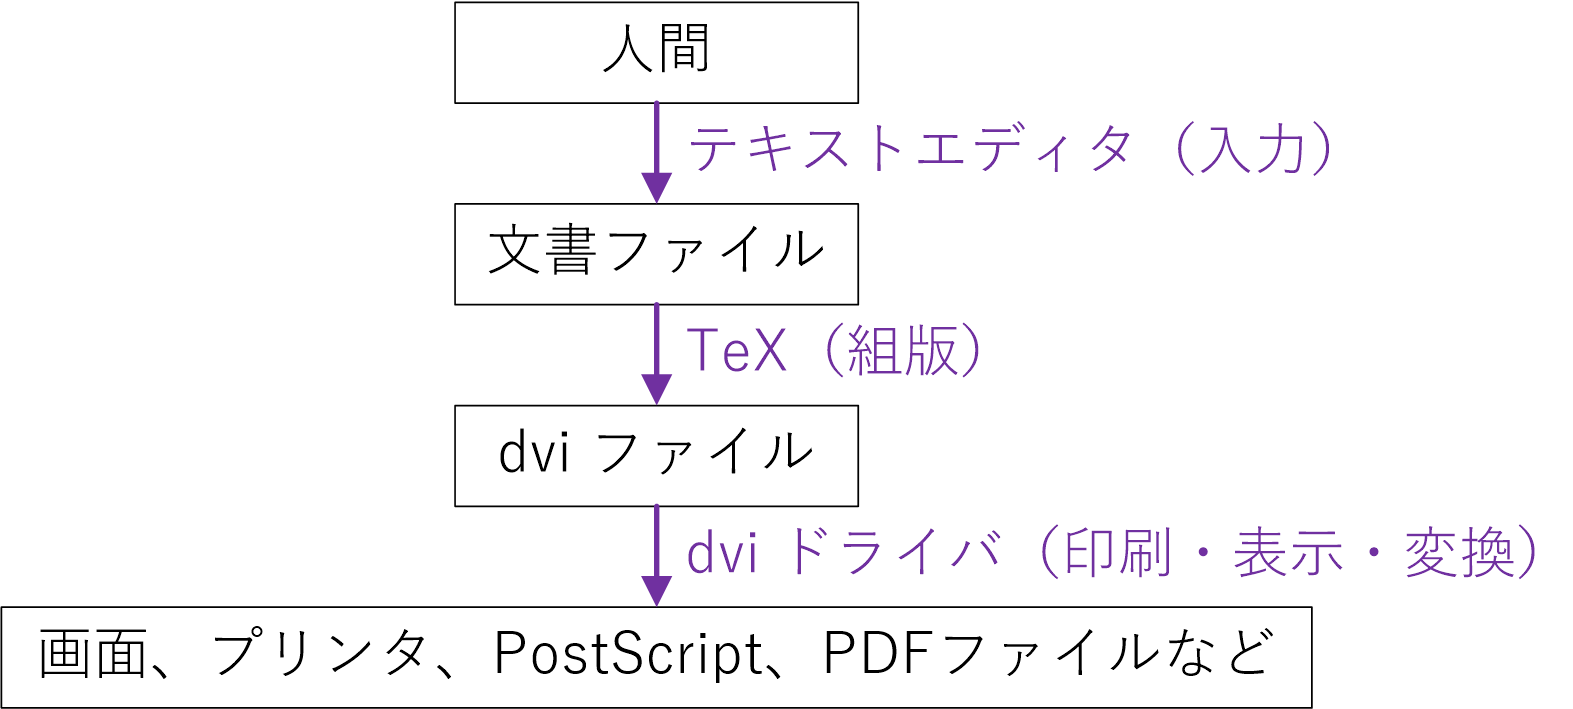
\includegraphics{./Part1/Fig/Fig01_01.PNG}}\caption{Part1で作成するスタンダードレイアウト}\label{Part1で作成するスタンダードレイアウト}\end{figure}\vspc{-3.00zw}
%%
%% 項:こんなことを学ぶ
%%----------------------------------------------------------------------------------------------------------%%
\subsection*{こんなことを学ぶ}
\vspc{-0.50zw}\begin{itemize}\setlength{\leftskip}{-1.00zw}%\setlength{\labelsep}{+1.00zw}
\item HTML5 の新要素
\item アウトライン
\end{itemize}\vspc{-1.50zw}
%%
%% 節:Part2:グリッドレイアウト
%%--------------------------------------------------------------------------------------------------------------------%%
\section{Part2:グリッドレイアウト}
ブラウザの横幅が変わるとブロックが自動で移動する可変グリッドレイアウトのサイトを作成する。
\vspc{-5.00pt}\begin{figure}[H]\centering\scalebox{0.37}{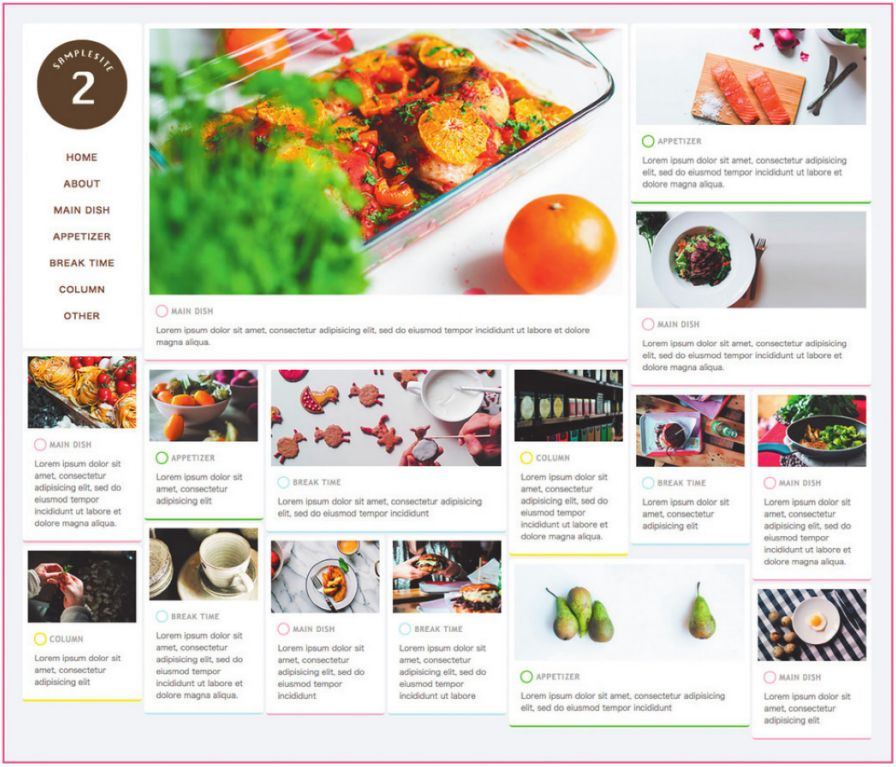
\includegraphics{./PART1/Fig/Fig01_02.PNG}}\caption{Part2で作成するグリッドレイアウト}\label{Part2で作成するグリッドレイアウト}\end{figure}\vspc{-3.00zw}
%%
%% 項:こんなことを学ぶ
%%----------------------------------------------------------------------------------------------------------%%
\subsection*{こんなことを学ぶ}
\vspc{-0.50zw}\begin{itemize}\setlength{\leftskip}{-1.00zw}%\setlength{\labelsep}{+1.00zw}
\item 可変グリッドレイアウトライブラリ
\item CSS アニメーション
\end{itemize}\vspc{-1.50zw}
%%
%% 節:Part3:グリッドレイアウト
%%--------------------------------------------------------------------------------------------------------------------%%
\section{Part3:シングルページレイアウト}
PC とスマートフォン両方に対応したシングルページレイアウトを作成する。
\vspc{-5.00pt}\begin{figure}[H]\centering\scalebox{0.45}{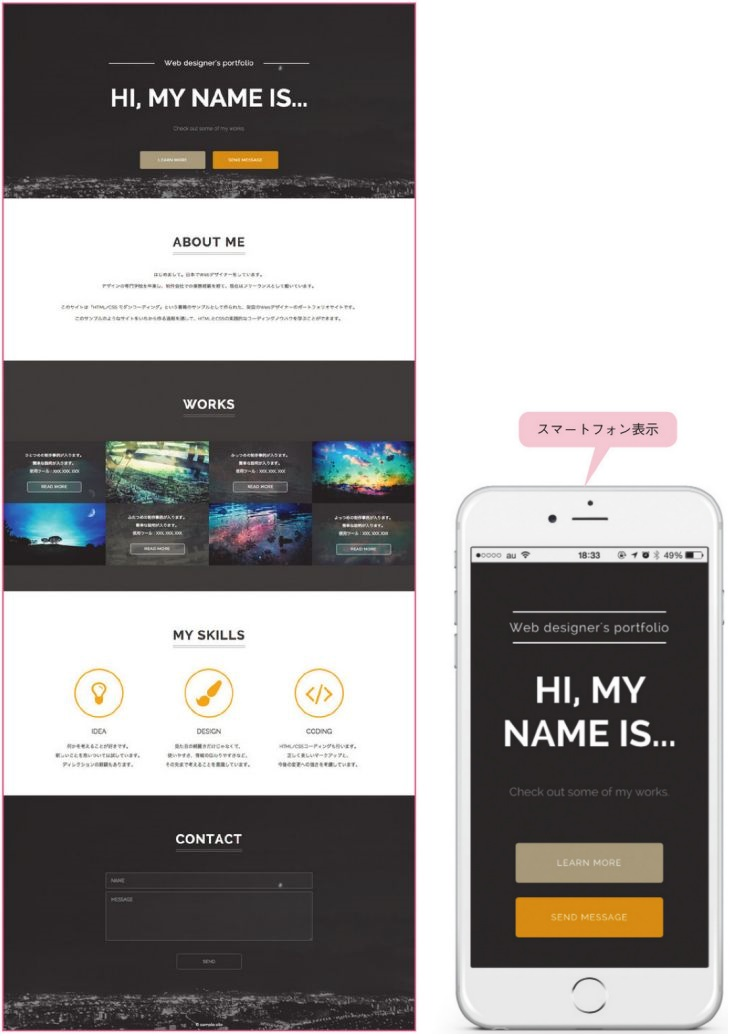
\includegraphics{./PART1/Fig/Fig01_03.PNG}}\caption{Part3で作成するシングルページレイアウト}\label{Part3で作成するシングルページレイアウト}\end{figure}\vspc{-3.00zw}
%%
%% 項:こんなことを学ぶ
%%----------------------------------------------------------------------------------------------------------%%
\subsection*{こんなことを学ぶ}
\vspc{-0.50zw}\begin{itemize}\setlength{\leftskip}{-1.00zw}%\setlength{\labelsep}{+1.00zw}
\item レスポンシブル Web デザイン
\item Web フォント
\end{itemize}\vspc{-1.50zw}
%%
%% 節:対応ブラウザ
%%--------------------------------------------------------------------------------------------------------------------%%
\section{対応ブラウザ}
本稿で作成するサイトの対応ブラウザは以下の通りである。
\vspc{-0.50zw}\begin{itemize}\setlength{\leftskip}{-1.00zw}%\setlength{\labelsep}{+1.00zw}
\item Internet Explorer 9 以上
\item Google Chrome
\item FireFox
\item Safari
\item シングルページレイアウトでのみ Mobile Safari、Chome to Mobile、Android Browser(Android 4.1 以降)
\end{itemize}\vspc{-0.50zw}
Internet Explore 8(以下、IE8 と記す)は 2016 年 1 月 12 日に Microsoft のサポート対象から外れ、セキュリティの更新やテクニカルサポートが提供されなくなったため、IE8 やそれ以下のレガシーブラウザは今後ますます使われなくなっていくことは明らかである。
そのため、本稿ではそれらのブラウザを対象ブラウザから除外している。\\

HTML5 に対応していないレガシーブラウザを除外することによって、コーディングに使える要素や機能がぐっと多くなるとともに、レガシーブラウザでの表示をフォローするための工夫も不要になるため、軽量で効率的なコーディングを行うことが可能となる。
これまでは比較的モダンとされていたようなコーディングが、IE8 のサポート終了以降も、もはやモダンではなくスタンダードとなっていくだろう。\\
%%
%% 節:コーディングの進め方
%%--------------------------------------------------------------------------------------------------------------------%%
\section{コーディングの進め方}
%%
%% 項:コーディングの前知識
%%----------------------------------------------------------------------------------------------------------%%
\subsection{コーディングの前知識}
本稿の解説で使用する HTML と CSS の各部の名称については以下の通りである。
\vspc{-0.50zw}\begin{longtable}{cl}
  \caption[]{HTML/CSSの各部名称\label{HTML/CSSの各部名称}}                                                                                                                \\[-1.30zw]\toprule
  \textgt{HTML} & \texttt{<\textcolor{orange}{要素名} \textcolor{blue}{属性}=}\verb|"|\texttt{\textcolor{red}{値}}\verb|"|\texttt{>テキスト</\textcolor{orange}{要素名}>} \\
  \textgt{CSS}  & \texttt{\textcolor{orange}{セレクタ} \{\,\textcolor{blue}{プロパティ}\hspc{+0.40pt}:\hspc{+1.00pt}\textcolor{red}{値}{;}\,\}}                           \\ \bottomrule
\end{longtable}\vspc{-0.90zw}
以下の CSS の基本的なセレクタについては、本稿の中では解説を省くことにする。
\vspc{-0.50zw}\begin{longtable}{ll}
  \caption[]{CSSの基本的なセレクタ\label{CSSの基本的なセレクタ}} \\[-1.30zw]\toprule
  \texttt{p}                       & 要素型                      \\ \midrule
  \texttt{{.}sample}\hspc{+4.00zw} & クラス\hspc{+3.00zw}        \\ \midrule
  \texttt{\#sample}                & id                          \\ \bottomrule
\end{longtable}\vspc{-0.90zw}
また、解説の中で、ある要素を示したい場合には CSS のセレクタと同様の表現を使用する。
%%
%% 項:コーディングする上でのポイント
%%----------------------------------------------------------------------------------------------------------%%
\subsection{コーディングする上でのポイント}
CSS コーディングの際に意識すると保守性が高まるポイントを紹介する。
本稿で扱うサンプルサイトも以下のポイントを踏まえて制作されている。
\vspc{-0.50zw}\begin{itemize}\setlength{\leftskip}{-1.00zw}%\setlength{\labelsep}{+1.00zw}
\item[\textcolor{red}{・}] \textcolor{red}{要素名にスタイルを指定しない} \\
  一度コーディングが終わっても、後から部分的な仕様の変更や対象ブラウザの変化などによって HTML のマークアップが変更される場合がある。
  そのような場合に要素名に対してスタイルを指定していると、HTML の編集と同時にセレクタを変更するために CSS ファイルも修正しなくてはならなくなる。
  但し、a要素、input要素、textarea要素など「その要素でないと機能が成り立たない」場合は要素の種類が変わる可能性が低いため、要素名に直接スタイルを指定するデメリットは小さくなる。
\item[\textcolor{red}{・}] \textcolor{red}{CSS のセレクタには ID ではなくクラスを使用する} \\
  CSS のセレクタにはクラスの他に ID も使用できるが、ID を避けた方がよい理由が 3 つある。\enlargethispage{0.50zw}
  \vspc{-0.00zw}\begin{itemize}\setlength{\leftskip}{-1.00zw}%\setlength{\labelsep}{+1.00zw}
  \item[\ajMaru{1}] \textbf{スタイルの使い回しができない} \\
    ID はクラスと異なり、同じページの中では 1 つの ID を複数回使えないという決まりがある。
    その為、ID にスタイルを指定してしまうと、そのスタイルは 1 つのページの中で一度までしか使用できなくなってしまう。
    最初のデザインではそれで問題なくても、後々の改善で同じデザインの要素を増やす必要が出てきた場合に問題となる。
  \item[\ajMaru{2}] \textbf{スタイルの上書きが難しい} \\
    CSS には詳細度という概念がある。
    詳細度とは、スタイルが適用される優先順位を決める仕組みである。詳しくは後述するが、ID はクラスよりも詳細度が高いので、ID で指定したスタイルは後からクラスで指定したスタイルで上書きすることができない。
  \item[\ajMaru{3}] \textbf{HTML や JavaScript と影響範囲を分離する} \\
    CSS セレクタはスタイルを指定したい要素を CSS から特定するためのものだが、要素の特定が必要な場合は CSS 以外でも発生する。
    HTML でページ内の特定の場所を指定してリンクする場合には ID を用いるし、JavaScript の処理で特定の 1 の要素を取得したい場合にも ID を使用すると効率がよい。
    前述した ID のルールに従い、同じ ID の要素が複数存在しないことを前提にできるので、絞り込みや重複確認をせずピンポイントで 1 つの要素を特定できるからである。
    そこで、ID は HTML、JavaScript からの特定に使用し、CSS セレクタは使用しないというようなルール付けをすると、影響範囲を分離できるので管理がし易くなる。
  \end{itemize}\vspc{-0.50zw}

\end{itemize}\vspc{-0.50zw}
%%
%% 項:リセット CSS について
%%----------------------------------------------------------------------------------------------------------%%
\subsection{リセット CSS について}
本稿で扱うサンプルサイトでは、解説の中で記述していく style.css の前に「リセットCSS」と呼ばれる CSS ファイルを読み込んでいる。\\

Web サイトを閲覧するブラウザは、それぞれ「ユーザエージェントスタイルシート(UAスタイルシート)」と呼ばれるスタイルシートを持っている。
ここには「h1要素は大きめの文字で太字」「p要素のまわりには間隔をあける」「ul要素にはリストマークを付ける」など、デフォルトで適用されるスタイルが記述されている。
そのおかげで、CSS が 1 行も書かれていない HTML 文書もある程度読み易く表示することができる。\\

便利な UA スタイルシートだが、次に挙げるような問題もある。
\vspc{-0.50zw}\begin{itemize}\setlength{\leftskip}{-1.00zw}%\setlength{\labelsep}{+1.00zw}
\item ブラウザごとに UA スタイルシートがあるため、適用される値のズレによって同じ HTML でもブラウザ間で表示が異なってしまう。
\item これから自分で記述するスタイルシートと UA スタイルシートの間に食い違いが存在すると、UA スタイルシートの不要なスタイルをわざわざ打ち消さなければならない。
\end{itemize}\vspc{-0.50zw}
これらの問題を解決してくれるのがリセット CSS である。
リセット CSS は各ブラウザの UA スタイルシートを一部リセットするための CSS で、この CSS を読み込むことで UA スタイルシートによる装飾がある程度まで打ち消され、ブラウザ間の差異をなくすことができる。\\

もう 1 つ似たものとして normalize.css という CSS もある。
これもブラウザ間での表示の差異をなくすという目的は reset.css と同じだが「リセット(初期化)」ではなく「ノーマライズ(統一する)」という名前の通り、UA スタイルシートの装飾を極力活かしながらブラウザ間の差異のみを埋めていくという点が異なる。\\

UA スタイルシートを活かせそうなサイトデザインであれば、こちらの CSS を読み込んだ方がコーディングの効率がよくなる場合がある。
本稿では、Part1 と Part2 では reset.css を、Part3 では normalize.css を利用している。

%% %%
%% 部:イントロダクション
%%------------------------------------------------------------------------------------------------------------------------------%%
\part{イントロダクション}
%%
%% 章:本稿で作成するサイト
%%------------------------------------------------------------------------------------------------------------------------------%%
\chapter{本稿で作成するサイト}
%%
%% 節:Part1:スタンダードレイアウト
%%--------------------------------------------------------------------------------------------------------------------%%
\section{Part1:スタンダードレイアウト}
Web サイトに一番多く見られるベーシックなレイアウトのサイトを作成する。
\vspc{-5.00pt}\begin{figure}[H]\centering\scalebox{0.48}{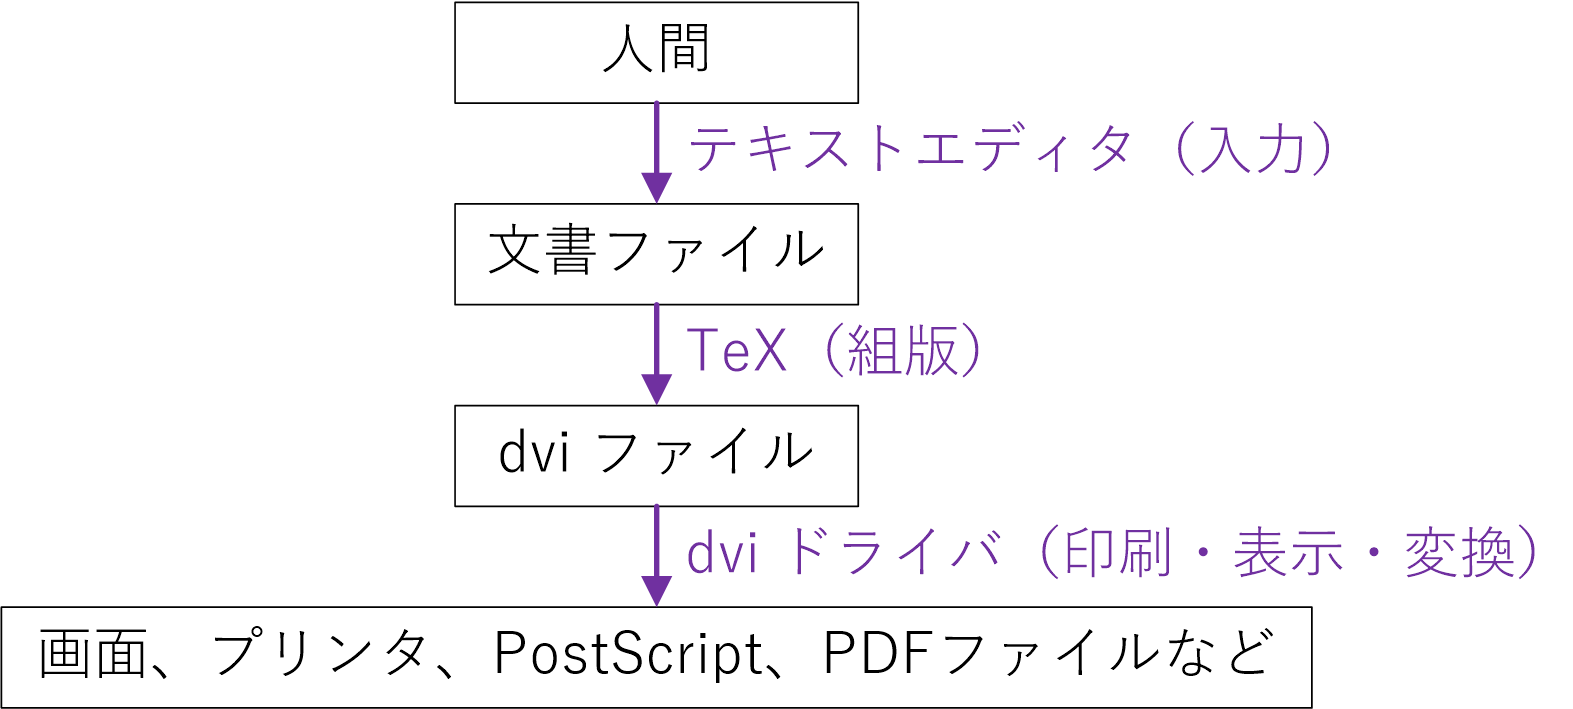
\includegraphics{./Part1/Fig/Fig01_01.PNG}}\caption{Part1で作成するスタンダードレイアウト}\label{Part1で作成するスタンダードレイアウト}\end{figure}\vspc{-3.00zw}
%%
%% 項:こんなことを学ぶ
%%----------------------------------------------------------------------------------------------------------%%
\subsection*{こんなことを学ぶ}
\vspc{-0.50zw}\begin{itemize}\setlength{\leftskip}{-1.00zw}%\setlength{\labelsep}{+1.00zw}
\item HTML5 の新要素
\item アウトライン
\end{itemize}\vspc{-1.50zw}
%%
%% 節:Part2:グリッドレイアウト
%%--------------------------------------------------------------------------------------------------------------------%%
\section{Part2:グリッドレイアウト}
ブラウザの横幅が変わるとブロックが自動で移動する可変グリッドレイアウトのサイトを作成する。
\vspc{-5.00pt}\begin{figure}[H]\centering\scalebox{0.37}{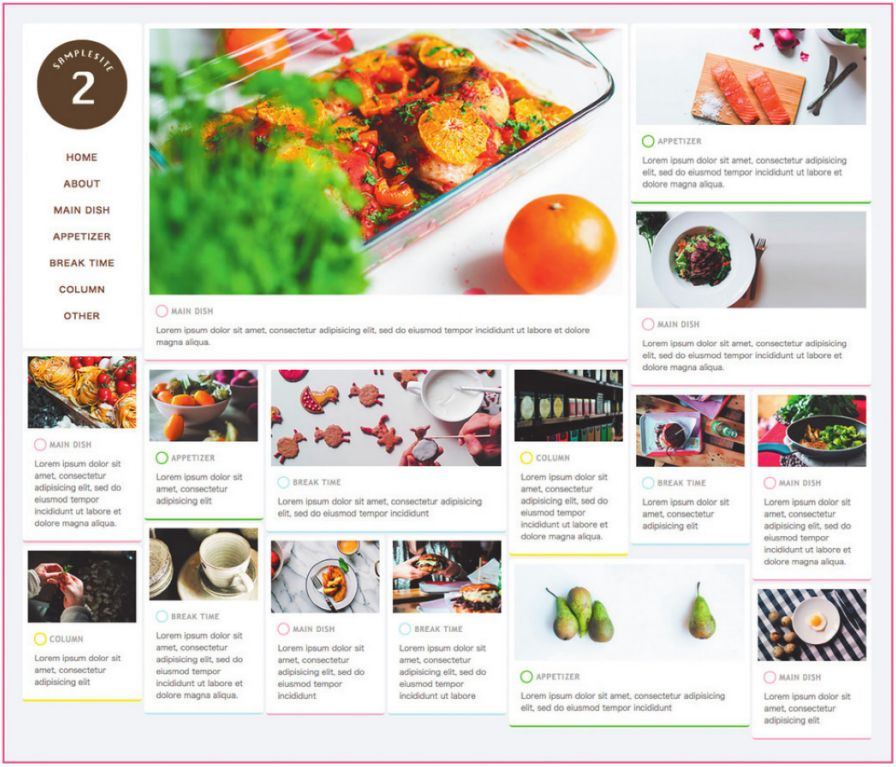
\includegraphics{./PART1/Fig/Fig01_02.PNG}}\caption{Part2で作成するグリッドレイアウト}\label{Part2で作成するグリッドレイアウト}\end{figure}\vspc{-3.00zw}
%%
%% 項:こんなことを学ぶ
%%----------------------------------------------------------------------------------------------------------%%
\subsection*{こんなことを学ぶ}
\vspc{-0.50zw}\begin{itemize}\setlength{\leftskip}{-1.00zw}%\setlength{\labelsep}{+1.00zw}
\item 可変グリッドレイアウトライブラリ
\item CSS アニメーション
\end{itemize}\vspc{-1.50zw}
%%
%% 節:Part3:グリッドレイアウト
%%--------------------------------------------------------------------------------------------------------------------%%
\section{Part3:シングルページレイアウト}
PC とスマートフォン両方に対応したシングルページレイアウトを作成する。
\vspc{-5.00pt}\begin{figure}[H]\centering\scalebox{0.45}{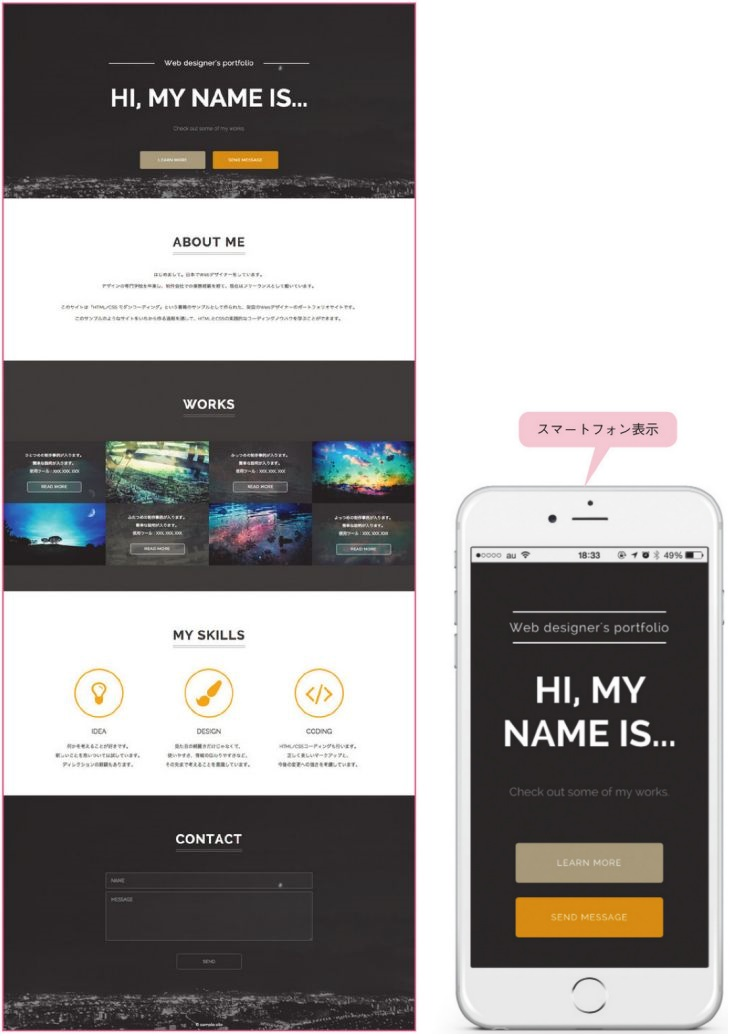
\includegraphics{./PART1/Fig/Fig01_03.PNG}}\caption{Part3で作成するシングルページレイアウト}\label{Part3で作成するシングルページレイアウト}\end{figure}\vspc{-3.00zw}
%%
%% 項:こんなことを学ぶ
%%----------------------------------------------------------------------------------------------------------%%
\subsection*{こんなことを学ぶ}
\vspc{-0.50zw}\begin{itemize}\setlength{\leftskip}{-1.00zw}%\setlength{\labelsep}{+1.00zw}
\item レスポンシブル Web デザイン
\item Web フォント
\end{itemize}\vspc{-1.50zw}
%%
%% 節:対応ブラウザ
%%--------------------------------------------------------------------------------------------------------------------%%
\section{対応ブラウザ}
本稿で作成するサイトの対応ブラウザは以下の通りである。
\vspc{-0.50zw}\begin{itemize}\setlength{\leftskip}{-1.00zw}%\setlength{\labelsep}{+1.00zw}
\item Internet Explorer 9 以上
\item Google Chrome
\item FireFox
\item Safari
\item シングルページレイアウトでのみ Mobile Safari、Chome to Mobile、Android Browser(Android 4.1 以降)
\end{itemize}\vspc{-0.50zw}
Internet Explore 8(以下、IE8 と記す)は 2016 年 1 月 12 日に Microsoft のサポート対象から外れ、セキュリティの更新やテクニカルサポートが提供されなくなったため、IE8 やそれ以下のレガシーブラウザは今後ますます使われなくなっていくことは明らかである。
そのため、本稿ではそれらのブラウザを対象ブラウザから除外している。\\

HTML5 に対応していないレガシーブラウザを除外することによって、コーディングに使える要素や機能がぐっと多くなるとともに、レガシーブラウザでの表示をフォローするための工夫も不要になるため、軽量で効率的なコーディングを行うことが可能となる。
これまでは比較的モダンとされていたようなコーディングが、IE8 のサポート終了以降も、もはやモダンではなくスタンダードとなっていくだろう。\\
%%
%% 節:コーディングの進め方
%%--------------------------------------------------------------------------------------------------------------------%%
\section{コーディングの進め方}
%%
%% 項:コーディングの前知識
%%----------------------------------------------------------------------------------------------------------%%
\subsection{コーディングの前知識}
本稿の解説で使用する HTML と CSS の各部の名称については以下の通りである。
\vspc{-0.50zw}\begin{longtable}{cl}
  \caption[]{HTML/CSSの各部名称\label{HTML/CSSの各部名称}}                                                                                                                \\[-1.30zw]\toprule
  \textgt{HTML} & \texttt{<\textcolor{orange}{要素名} \textcolor{blue}{属性}=}\verb|"|\texttt{\textcolor{red}{値}}\verb|"|\texttt{>テキスト</\textcolor{orange}{要素名}>} \\
  \textgt{CSS}  & \texttt{\textcolor{orange}{セレクタ} \{\,\textcolor{blue}{プロパティ}\hspc{+0.40pt}:\hspc{+1.00pt}\textcolor{red}{値}{;}\,\}}                           \\ \bottomrule
\end{longtable}\vspc{-0.90zw}
以下の CSS の基本的なセレクタについては、本稿の中では解説を省くことにする。
\vspc{-0.50zw}\begin{longtable}{ll}
  \caption[]{CSSの基本的なセレクタ\label{CSSの基本的なセレクタ}} \\[-1.30zw]\toprule
  \texttt{p}                       & 要素型                      \\ \midrule
  \texttt{{.}sample}\hspc{+4.00zw} & クラス\hspc{+3.00zw}        \\ \midrule
  \texttt{\#sample}                & id                          \\ \bottomrule
\end{longtable}\vspc{-0.90zw}
また、解説の中で、ある要素を示したい場合には CSS のセレクタと同様の表現を使用する。
%%
%% 項:コーディングする上でのポイント
%%----------------------------------------------------------------------------------------------------------%%
\subsection{コーディングする上でのポイント}
CSS コーディングの際に意識すると保守性が高まるポイントを紹介する。
本稿で扱うサンプルサイトも以下のポイントを踏まえて制作されている。
\vspc{-0.50zw}\begin{itemize}\setlength{\leftskip}{-1.00zw}%\setlength{\labelsep}{+1.00zw}
\item[\textcolor{red}{・}] \textcolor{red}{要素名にスタイルを指定しない} \\
  一度コーディングが終わっても、後から部分的な仕様の変更や対象ブラウザの変化などによって HTML のマークアップが変更される場合がある。
  そのような場合に要素名に対してスタイルを指定していると、HTML の編集と同時にセレクタを変更するために CSS ファイルも修正しなくてはならなくなる。
  但し、a要素、input要素、textarea要素など「その要素でないと機能が成り立たない」場合は要素の種類が変わる可能性が低いため、要素名に直接スタイルを指定するデメリットは小さくなる。
\item[\textcolor{red}{・}] \textcolor{red}{CSS のセレクタには ID ではなくクラスを使用する} \\
  CSS のセレクタにはクラスの他に ID も使用できるが、ID を避けた方がよい理由が 3 つある。\enlargethispage{0.50zw}
  \vspc{-0.00zw}\begin{itemize}\setlength{\leftskip}{-1.00zw}%\setlength{\labelsep}{+1.00zw}
  \item[\ajMaru{1}] \textbf{スタイルの使い回しができない} \\
    ID はクラスと異なり、同じページの中では 1 つの ID を複数回使えないという決まりがある。
    その為、ID にスタイルを指定してしまうと、そのスタイルは 1 つのページの中で一度までしか使用できなくなってしまう。
    最初のデザインではそれで問題なくても、後々の改善で同じデザインの要素を増やす必要が出てきた場合に問題となる。
  \item[\ajMaru{2}] \textbf{スタイルの上書きが難しい} \\
    CSS には詳細度という概念がある。
    詳細度とは、スタイルが適用される優先順位を決める仕組みである。詳しくは後述するが、ID はクラスよりも詳細度が高いので、ID で指定したスタイルは後からクラスで指定したスタイルで上書きすることができない。
  \item[\ajMaru{3}] \textbf{HTML や JavaScript と影響範囲を分離する} \\
    CSS セレクタはスタイルを指定したい要素を CSS から特定するためのものだが、要素の特定が必要な場合は CSS 以外でも発生する。
    HTML でページ内の特定の場所を指定してリンクする場合には ID を用いるし、JavaScript の処理で特定の 1 の要素を取得したい場合にも ID を使用すると効率がよい。
    前述した ID のルールに従い、同じ ID の要素が複数存在しないことを前提にできるので、絞り込みや重複確認をせずピンポイントで 1 つの要素を特定できるからである。
    そこで、ID は HTML、JavaScript からの特定に使用し、CSS セレクタは使用しないというようなルール付けをすると、影響範囲を分離できるので管理がし易くなる。
  \end{itemize}\vspc{-0.50zw}

\end{itemize}\vspc{-0.50zw}
%%
%% 項:リセット CSS について
%%----------------------------------------------------------------------------------------------------------%%
\subsection{リセット CSS について}
本稿で扱うサンプルサイトでは、解説の中で記述していく style.css の前に「リセットCSS」と呼ばれる CSS ファイルを読み込んでいる。\\

Web サイトを閲覧するブラウザは、それぞれ「ユーザエージェントスタイルシート(UAスタイルシート)」と呼ばれるスタイルシートを持っている。
ここには「h1要素は大きめの文字で太字」「p要素のまわりには間隔をあける」「ul要素にはリストマークを付ける」など、デフォルトで適用されるスタイルが記述されている。
そのおかげで、CSS が 1 行も書かれていない HTML 文書もある程度読み易く表示することができる。\\

便利な UA スタイルシートだが、次に挙げるような問題もある。
\vspc{-0.50zw}\begin{itemize}\setlength{\leftskip}{-1.00zw}%\setlength{\labelsep}{+1.00zw}
\item ブラウザごとに UA スタイルシートがあるため、適用される値のズレによって同じ HTML でもブラウザ間で表示が異なってしまう。
\item これから自分で記述するスタイルシートと UA スタイルシートの間に食い違いが存在すると、UA スタイルシートの不要なスタイルをわざわざ打ち消さなければならない。
\end{itemize}\vspc{-0.50zw}
これらの問題を解決してくれるのがリセット CSS である。
リセット CSS は各ブラウザの UA スタイルシートを一部リセットするための CSS で、この CSS を読み込むことで UA スタイルシートによる装飾がある程度まで打ち消され、ブラウザ間の差異をなくすことができる。\\

もう 1 つ似たものとして normalize.css という CSS もある。
これもブラウザ間での表示の差異をなくすという目的は reset.css と同じだが「リセット(初期化)」ではなく「ノーマライズ(統一する)」という名前の通り、UA スタイルシートの装飾を極力活かしながらブラウザ間の差異のみを埋めていくという点が異なる。\\

UA スタイルシートを活かせそうなサイトデザインであれば、こちらの CSS を読み込んだ方がコーディングの効率がよくなる場合がある。
本稿では、Part1 と Part2 では reset.css を、Part3 では normalize.css を利用している。

%%
%% 章:ベースのコーディング
%%------------------------------------------------------------------------------------------------------------------------------%%
\chapter{ベースのコーディング}
それぞれの箇所のコーディングに入る前に、サイト全体に影響する部分のコーディングを行う。
%%
%% 節:ファイル構成
%%--------------------------------------------------------------------------------------------------------------------%%
\section{ファイル構成}
\begin{wrapfigure}{r}{19.00zw}
  \vspace*{-\intextsep}
  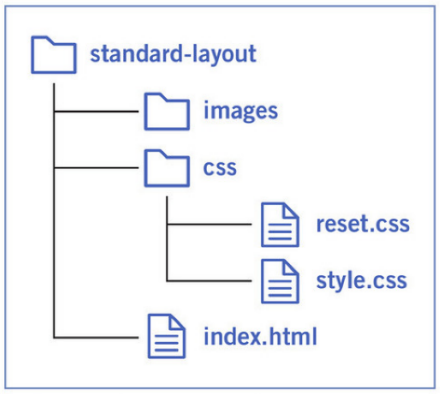
\includegraphics[width=19.00zw]{./PART2/Fig/Fig01_03.PNG}
\end{wrapfigure}
今回制作するスタンダードレイアウトサイトのファイル構成を確認しておく。
ベースになるファイルは、翔泳社のダウンロードサイト\footnote{http://www.shoeisha.co.jp/book/download/9784798141572}で配布されている。
ファイルをダウンロードしたら css/reset.css と image/ 以下のファイルはダウンロードしたファイルをそのまま利用する。\\

メインとなる index.html と css/style.css をこれから記述していく。
%%
%% 節:要素とサイズの確認
%%--------------------------------------------------------------------------------------------------------------------%%
\section{要素とサイズの確認}

\end{document}
